\section{实验结果与分析}

\subsection{二维数据降至一维}

生成$N=20$个数据点,满足多元高斯分布,降维至一维效果如图\ref{1},\ref{2},\ref{3}所示。

\begin{figure}[htbp]
    \begin{minipage}[t]{0.3\linewidth}
        \centering
        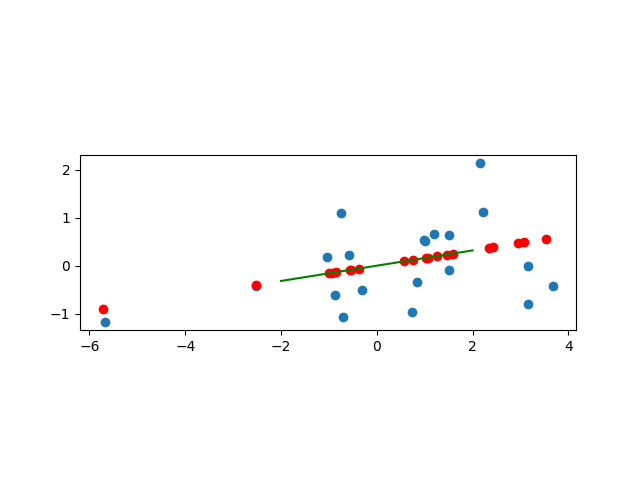
\includegraphics[width=\textwidth]{figures/Figure_4.png}
        \caption{$\mu=0$,$\sigma=5,1$,相关系数$=1$}
        \label{1}
    \end{minipage}
    \begin{minipage}[t]{0.3\linewidth}
        \centering
        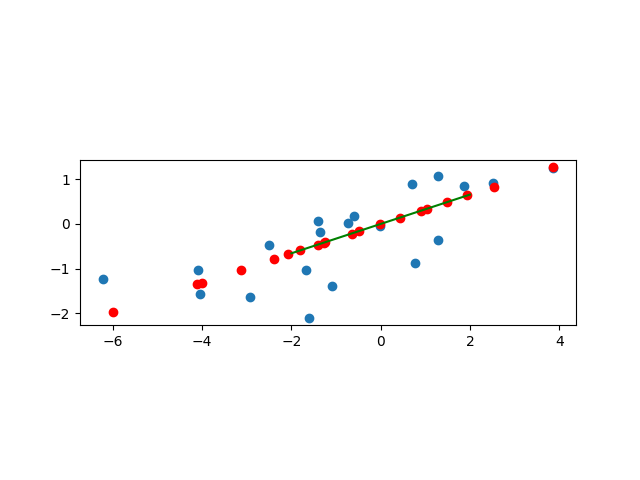
\includegraphics[width=\textwidth]{figures/Figure_5.png}
        \caption{$\mu=0$,$\sigma=6,1$,相关系数$=2$}
        \label{2}
    \end{minipage}
    \begin{minipage}[t]{0.3\linewidth}
        \centering
        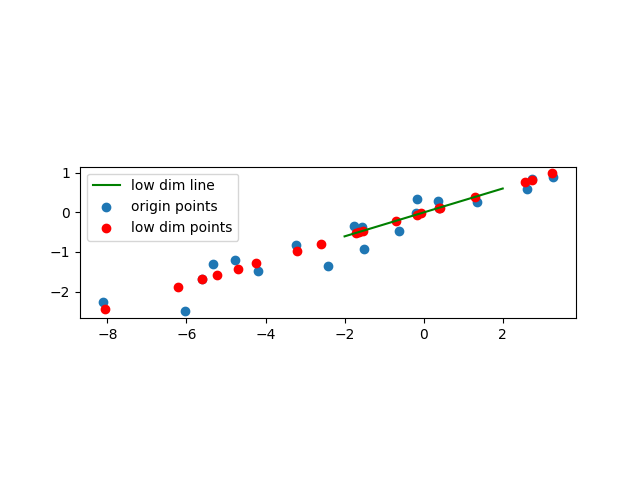
\includegraphics[width=\textwidth]{figures/Figure_6.png}
        \caption{$\mu=0$,$\sigma=10,1$,相关系数$=3$}
        \label{3}
    \end{minipage}
\end{figure}

生成$N=100$个数据点,满足多元高斯分布,降维至一维效果如图\ref{4},\ref{5},\ref{6}所示。

\begin{figure}[htbp]
    \begin{minipage}[t]{0.3\linewidth}
        \centering
        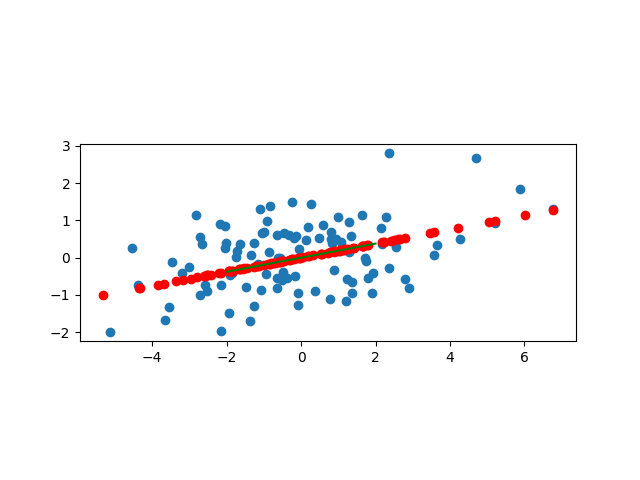
\includegraphics[width=\textwidth]{figures/Figure_1.png}
        \caption{$\mu=0$,$\sigma=5,1$,相关系数$=1$}
        \label{4}
    \end{minipage}
    \begin{minipage}[t]{0.3\linewidth}
        \centering
        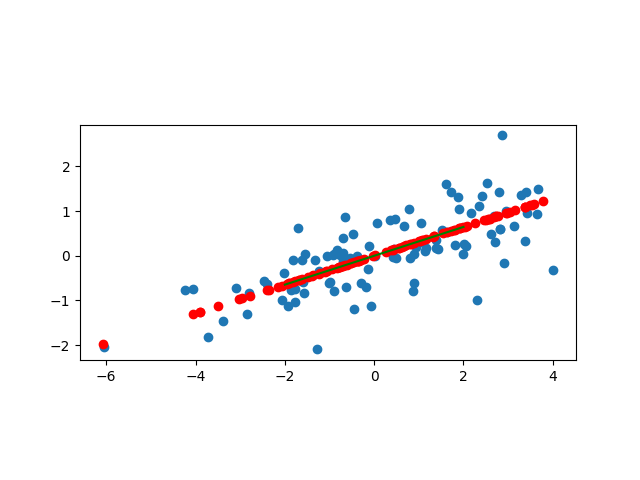
\includegraphics[width=\textwidth]{figures/Figure_2.png}
        \caption{$\mu=0$,$\sigma=6,1$,相关系数$=2$}
        \label{5}
    \end{minipage}
    \begin{minipage}[t]{0.3\linewidth}
        \centering
        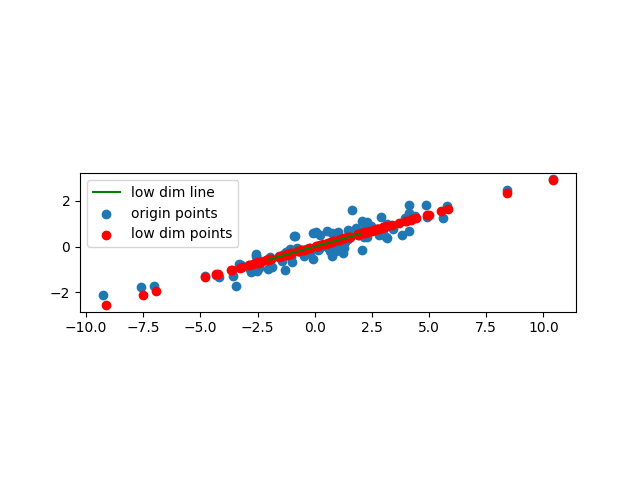
\includegraphics[width=\textwidth]{figures/Figure_3.png}
        \caption{$\mu=0$,$\sigma=10,1$,相关系数$=3$}
        \label{6}
    \end{minipage}
\end{figure}

其中绿色的直线是失真最小特征向量所在直线,红色的点是原始数据降维后的数据点。

\subsection{二维数据旋转}

$N=20$时,数据旋转效果如图\ref{7},\ref{8},\ref{9}。其中蓝色的相互正交的直线是旋转后新的坐标轴。

\begin{figure}[htbp]
    \begin{minipage}[t]{0.3\linewidth}
        \centering
        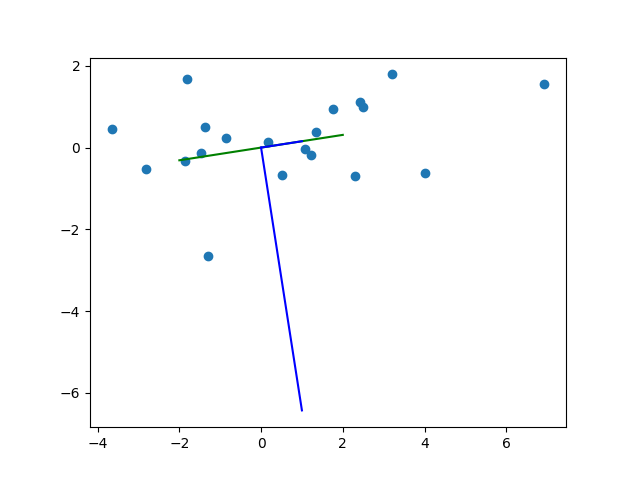
\includegraphics[width=\textwidth]{figures/Figure_7.png}
        \caption{$\mu=0$,$\sigma=5,1$,相关系数$=1$}
        \label{7}
    \end{minipage}
    \begin{minipage}[t]{0.3\linewidth}
        \centering
        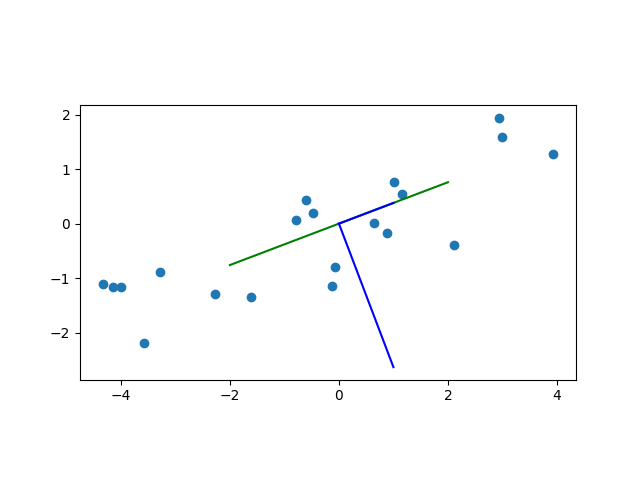
\includegraphics[width=\textwidth]{figures/Figure_8.png}
        \caption{$\mu=0$,$\sigma=6,1$,相关系数$=2$}
        \label{8}
    \end{minipage}
    \begin{minipage}[t]{0.3\linewidth}
        \centering
        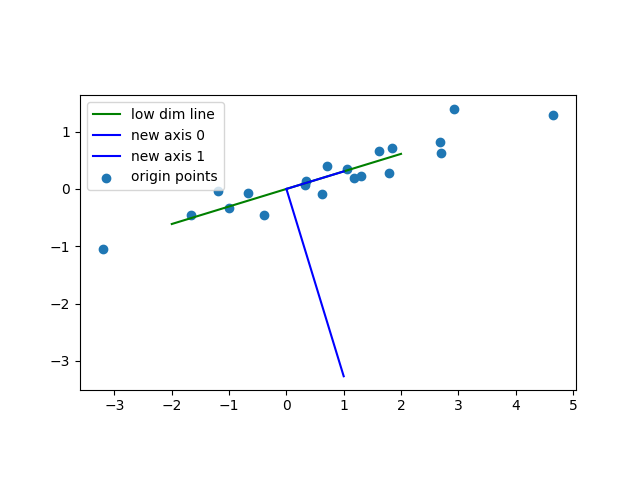
\includegraphics[width=\textwidth]{figures/Figure_9.png}
        \caption{$\mu=0$,$\sigma=10,1$,相关系数$=3$}
        \label{9}
    \end{minipage}
\end{figure}

$N=100$时,数据旋转效果如图\ref{10},\ref{11},\ref{12}。其中蓝色的相互正交的直线是旋转后新的坐标轴。

\begin{figure}[htbp]
    \begin{minipage}[t]{0.3\linewidth}
        \centering
        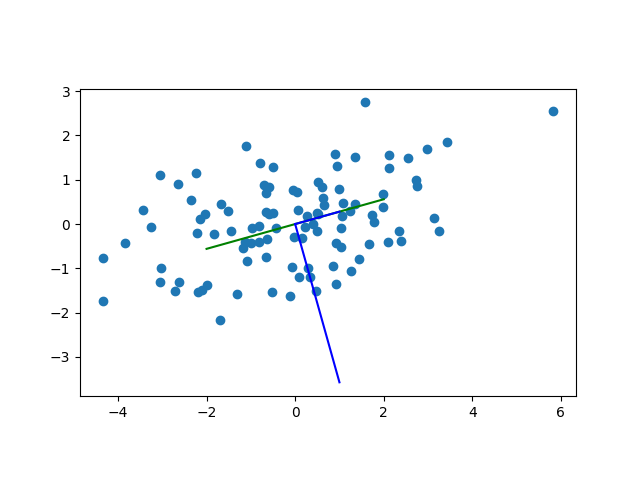
\includegraphics[width=\textwidth]{figures/Figure_10.png}
        \caption{$\mu=0$,$\sigma=5,1$,相关系数$=1$}
        \label{10}
    \end{minipage}
    \begin{minipage}[t]{0.3\linewidth}
        \centering
        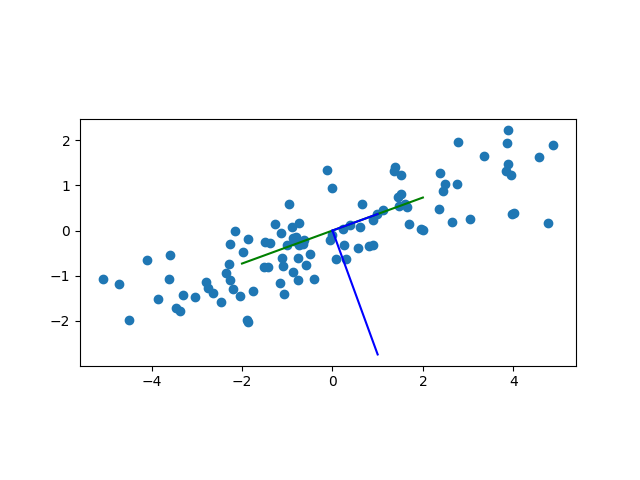
\includegraphics[width=\textwidth]{figures/Figure_11.png}
        \caption{$\mu=0$,$\sigma=6,1$,相关系数$=2$}
        \label{11}
    \end{minipage}
    \begin{minipage}[t]{0.3\linewidth}
        \centering
        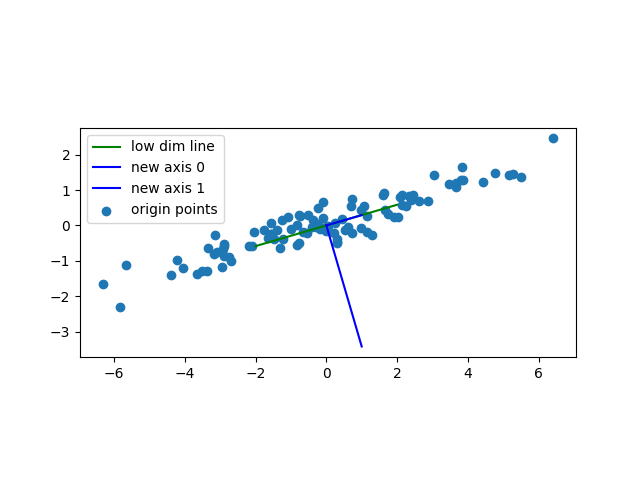
\includegraphics[width=\textwidth]{figures/Figure_12.png}
        \caption{$\mu=0$,$\sigma=10,1$,相关系数$=3$}
        \label{12}
    \end{minipage}
\end{figure}

\subsection{人脸数据降维}

为降低运算量,读入图片时使用Pillow的convert("L")转换为灰度图,其计算方式\cite{pillow}为
\begin{equation}
    L=\dfrac{299}{1000}R+\dfrac{587}{1000}G+\dfrac{114}{1000}B
    \label{L}
\end{equation}
可见其中的绿色分量占到一半以上,因此以下展示的图片呈绿色属于正常现象。

原始图片如图\ref{origin-img}。

\begin{figure}[htbp]
    \centering
    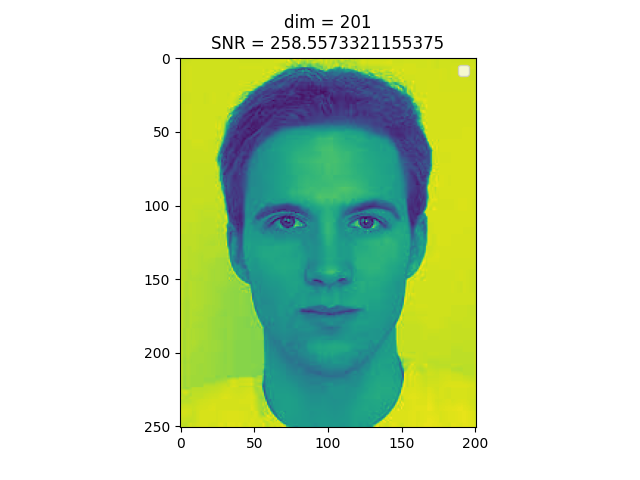
\includegraphics[width=0.3\textwidth]{figures/Figure_13.png}
    \caption{原始人脸图片,根据式\ref{L},图片泛绿是正常现象}
    \label{origin-img}
\end{figure}

分别降维到$M=100$,$M=50$,$M=20$,降维后重建的图片和信噪比如图\ref{m100},\ref{m50},\ref{m20}所示。

\begin{figure}[htbp]
    \begin{minipage}[t]{0.3\linewidth}
        \centering
        
\includegraphics[width=\textwidth]{figures/Figure_14.png}
        \caption{降维到$M=100$,信噪比$SNR=49.94$}
        \label{m100}
    \end{minipage}
    \begin{minipage}[t]{0.3\linewidth}
        \centering
        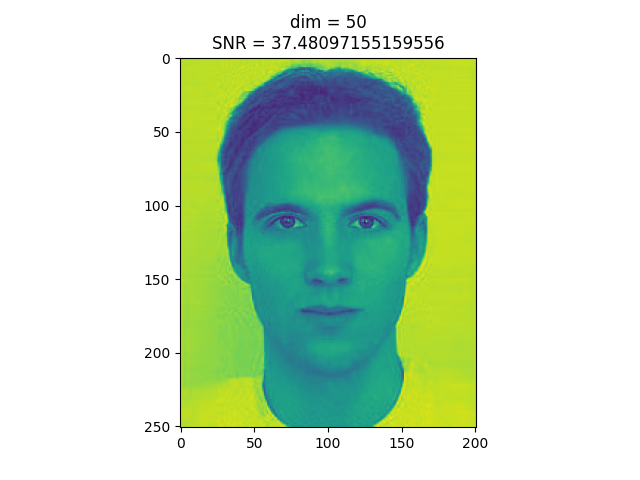
\includegraphics[width=\textwidth]{figures/Figure_15.png}
        \caption{降维到$M=50$,信噪比$SNR=37.48$}
        \label{m50}
    \end{minipage}
    \begin{minipage}[t]{0.3\linewidth}
        \centering
        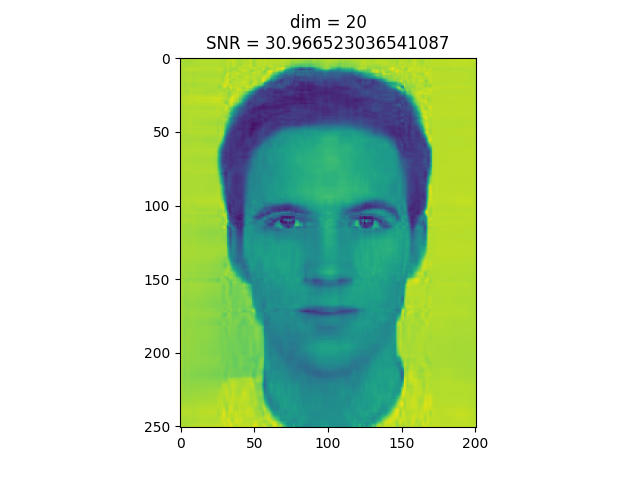
\includegraphics[width=\textwidth]{figures/Figure_16.png}
        \caption{降维到$M=20$,信噪比$SNR=30.97$}
        \label{m20}
    \end{minipage}
\end{figure}

可见已经有些模糊,继续降维到$M=15$,$M=10$,$M=5$,降维后重建的图片和信噪比如图\ref{m15},\ref{m20},\ref{m5}所示。

\begin{figure}[htbp]
    \begin{minipage}[t]{0.3\linewidth}
        \centering
        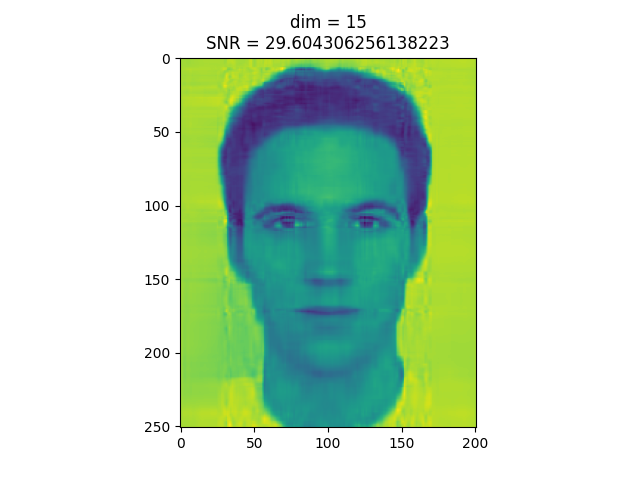
\includegraphics[width=\textwidth]{figures/Figure_17.png}
        \caption{降维到$M=15$,信噪比$SNR=29.60$}
        \label{m15}
    \end{minipage}
    \begin{minipage}[t]{0.3\linewidth}
        \centering
        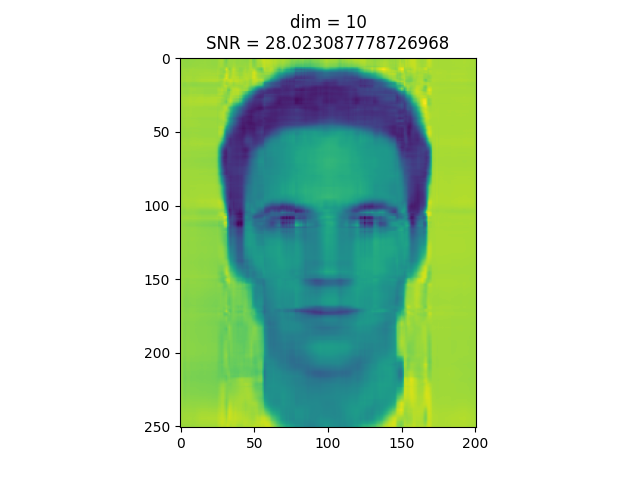
\includegraphics[width=\textwidth]{figures/Figure_18.png}
        \caption{降维到$M=10$,信噪比$SNR=28.02$}
        \label{m10}
    \end{minipage}
    \begin{minipage}[t]{0.3\linewidth}
        \centering
        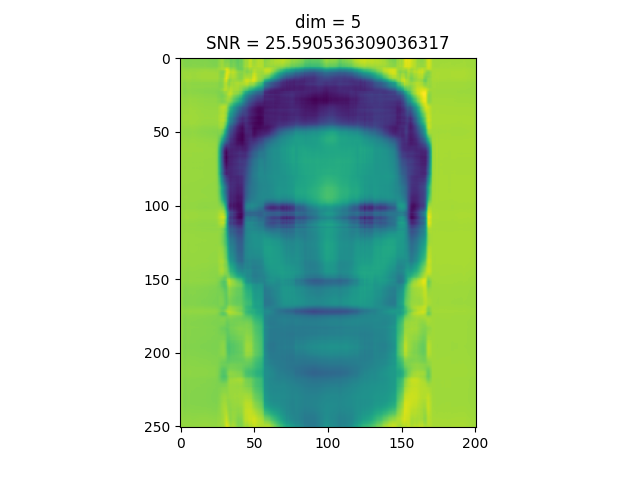
\includegraphics[width=\textwidth]{figures/Figure_19.png}
        \caption{降维到$M=5$,信噪比$SNR=25.59$}
        \label{m5}
    \end{minipage}
\end{figure}

可见降维已经使图片模糊不清,信噪比逐渐降低。降维的维度$M$和对应信噪比$SNR$关系如图\ref{snr}。

\begin{figure}[htbp]
    \centering
    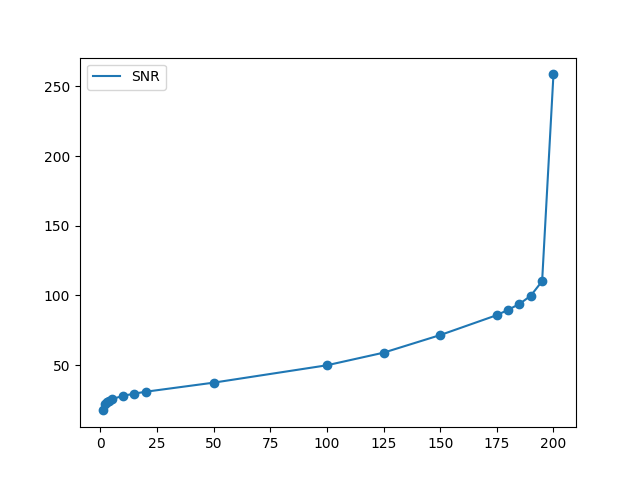
\includegraphics[width=0.7\textwidth]{figures/Figure_20.png}
    \caption{维度$M$和对应信噪比$SNR$关系}
    \label{snr}
\end{figure}

可见随着维度的下降,信噪比也在下降,这相当于图片越来越不清晰,与观测结果一致。
